\documentclass{article}
\usepackage[utf8]{inputenc}

\title{Kalman Filter for Missile State Estimation}
\author{Alonzo Lopez}
\date{March 10, 2021}
\usepackage{graphicx}
\usepackage{amsmath}
\begin{document}

\maketitle

\section{Abstract}
A continuous-time Kalman Filter is implemented to estimate the relative states in a missile intercept operation. The filter's performance is first verified via
Monte Carlo simulation of a Gauss-Markov process driven by a random forcing function with an exponential correlation. The filter's robustness is then confirmed in 
a second Monte Carlo simulation where the dynamic model is driven by a random telegraph signal instead of the random forcing function.

\section{Introduction}
The missile intercept problem illustrated in Figure \ref{MissileIntercept} features a pursuer attempting to close the distance between itself and a maneuvering target. 
This problem has two parts: estimation and control. The Kalman Filter detailed in this paper solves the estimation problem given a stochastic process model and 
sensor noise model. 

\begin{figure}
    \centering
    \includegraphics[width=1\textwidth]{missile_intercept.png}
    \caption{Missile Intercept Illustration.}
    \label{MissileIntercept}
\end{figure}

\section{The Dynamic Model}
The dynamics of the problem are 
\begin{equation}
    \begin{split}
        \dot y & = v \\
        \dot v & = a_P - a_T    
    \end{split}
\end{equation}
where $a_P$, the acceleration of the Pursuer, is known to be zero. The input, $a_T$, is the target acceleration and is treated as a random forcing function with an exponential correlation,
\begin{equation}
    \begin{split}
        E[a_T] & = 0 \\
        E[a_T(t)a_T(s)] & = E[a_T^2] e^{\frac{-|t-s|}{\tau}}
    \end{split}
\end{equation}
The scalar, $\tau$, is the correlation time. The initial lateral position, $y(t_0)$, is zero by definition. The initial lateral velocity, $v(t_0)$, is random and assumed to 
be the result of launching error:

\begin{center}
    \begin{tabular}{c c c c c c c c }
        $E[y(t_0)]$   & $=0$ & \; & $E[v(t_0)]$ & $= 0$ & &  &  \\
        $E[y(t_0)^2]$ & $=0$ & \; & $E[y(t_0)v(t_0)]$ & $=0$& & $E[v(t_0)^2]$ &  = given
    \end{tabular}
\end{center}

The measurement, $z$, consists of a line-of-sight angle, $\theta$. For $|\theta|<<1$,
\begin{equation}
    \theta \approx \frac{y}{V_c (t_f - t)}
\end{equation}

It will also be assumed that $z$ is corrupted by fading and scintiallation noise so that
\begin{equation}
    \begin{split}
        z & = \theta + n \\
        E[n(t)] & = 0 \\
        E[n(t)n(\tau)] & = V\delta(t-\tau) = \begin{bmatrix}
            R_1 + \frac{R_2}{(t_f - t)^2}\delta(t-\tau)
        \end{bmatrix}
    \end{split}
\end{equation}
The process noise spectral density, $W$, is 
\begin{equation}
    W = G E[a_T^2] G^T = \begin{bmatrix}
        0 & 0 & 0 \\
        0 & 0 & 0 \\
        0 & 0 & E[a_T^2]
    \end{bmatrix}
\end{equation}
Given the above, the state-space equations for the process and measurement are
\begin{equation}\label{SS_process}
    \begin{bmatrix}
        \dot y \\
        \dot v \\
        \dot a_T
    \end{bmatrix} = 
    \underbrace{
        \begin{bmatrix}
            0 & 1 & 0 \\
            0 & 0 & -1 \\
            0 & 0 & -\frac{1}{\tau}
        \end{bmatrix}
    }_{F} 
    \underbrace{
        \begin{bmatrix}
            y \\
            v \\
            a_T
        \end{bmatrix}
    }_{x} + 
    \underbrace{
        \begin{bmatrix}
            0 \\ 
            1 \\
            0
        \end{bmatrix}
    }_{B} a_P + 
    \underbrace{
        \begin{bmatrix}
            0 \\
            0 \\
            1
        \end{bmatrix}
    }_{G} w_{a_T}
\end{equation}
\begin{equation}\label{SS_measurement}
    z = 
    \underbrace{
        \begin{bmatrix}
            \frac{1}{Vc(t_f -t)} & 0 & 0
        \end{bmatrix}
    }_{H}
    \begin{bmatrix}
        y \\
        v \\
        a_T
    \end{bmatrix} + n
\end{equation}
The following values are used to simulate the above model.
\begin{center}
    \begin{tabular}{c c c c}
        $V_c = 300 \frac{ft}{sec}$ & $E[a_T^2] = (100 \frac{ft}{sec^2})^2$ & $t_f = 10 sec$ & $R_1 = 15 \times 10^{-6} \frac{rad^2}{sec}$ \\
        $R_2 = 1.67 \times 10^{-3} \frac{rad^2}{sec^3}$ & & $\tau = 2 sec$ & $b = 1.52 \times 10^{-2}$
    \end{tabular}
\end{center}
\section{The Kalman Filter Algorithm}
The continuous-time Kalman Filter has the form
\begin{equation}
    \begin{split}
        \dot{\hat y} & = \hat v + K_1 \underbrace{\begin{pmatrix}z - \frac{\hat y}{V_c(t_f - t)}\end{pmatrix}}_{residual} \\
        \dot{\hat v} & = -\hat{a}_T + K_2 \begin{pmatrix}z - \frac{\hat y}{V_c(t_f - t)}\end{pmatrix} \\
        \dot{\hat{a}}_T & = - \frac{\hat{a}_T}{\tau} + K_3 \begin{pmatrix}z - \frac{\hat y}{V_c(t_f - t)} \end{pmatrix}
    \end{split}
\end{equation}
Where the gains are
\begin{equation}
    \begin{split}
        K_1 & = \frac{p_{11}}{V_c R_1 (t_f - t) + \frac{V_c R_2}{t_f - t}} \\
        K_2 & = \frac{p_{12}}{V_c R_1 (t_f - t) + \frac{V_c R_2}{t_f - t}} \\
        K_3 & = \frac{p_{13}}{V_c R_1 (t_f - t) + \frac{V_c R_2}{t_f - t}} 
    \end{split}
\end{equation}
The scalars, $p_{ij}$,are the (i, j) elements of the error covariance matrix that is propagated by the Ricatti equation,
\begin{equation}
    \dot P = F P + P F^T - \frac{1}{V_c^2 R_1 (t_f - t)^2 + V_c^2 R_2}P \bar{H}^T \bar{H} P + W
\end{equation}
where $\bar{H} = \begin{bmatrix}
    1 & 0 & 0
\end{bmatrix}$.
\section{Simulation Results and Discussion}
\subsection{Simulation Initialization}
Every simulation run has its true states, $y$, $v$, and $a_T$, initialized by drawing from a zero-mean Gaussian
with covariance values as indicated along the diagonal of the below initial covariance
\begin{equation}
    P(0) = 
    \begin{bmatrix}
        \underbrace{0}_{E[y(t_0)^2]} & 0 & 0 \\
        0 & \underbrace{\begin{pmatrix}200 \frac{ft}{sec})^2 \end{pmatrix}}_{E[v(t_0)^2]} & 0 \\
        0 & 0 & \underbrace{\begin{pmatrix}100 \frac{ft}{sec^2})^2 \end{pmatrix}}_{E[a_T^2]}
    \end{bmatrix}
\end{equation}
The true states are propagated via Euler integration using (\ref{SS_process}), and a noise sequence is generated to provide the simulation values of $w_{a_T}$. 
For each discrete-time instant in the simulation, the sensor measurement is simulated using (\ref{SS_measurement}).
\subsection{Analysis of One Realization}
\begin{figure}
    \centering
    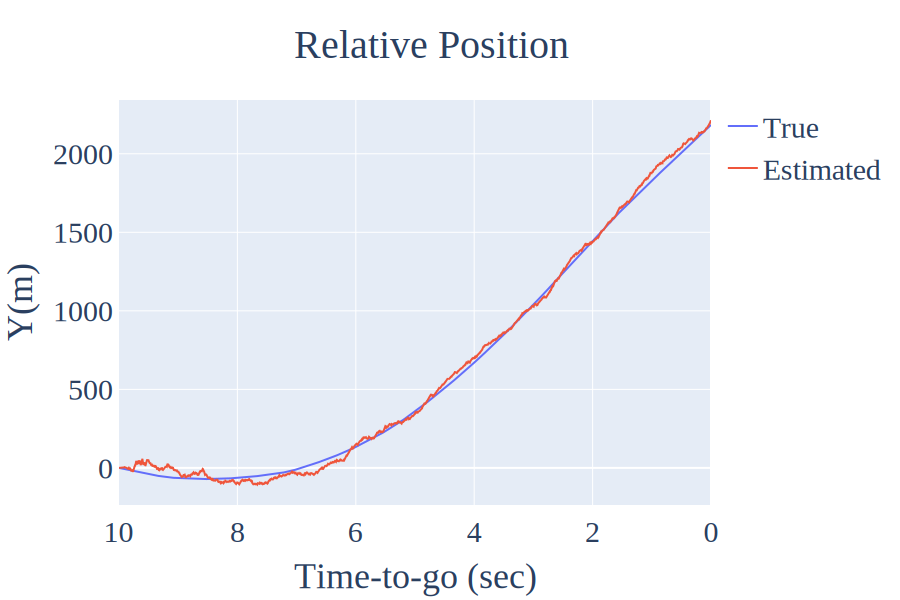
\includegraphics[width=1\textwidth]{figy.png}
    \caption{The true and estimated relative distance along y between the pursuer and target.}
    \label{Relative_Position}
\end{figure}

\begin{figure}
    \centering
    \includegraphics[width=1\textwidth]{figv.png}
    \caption{The true and estimated relative velocity along y between the pursuer and target.}
    \label{Relative_Velocity}
\end{figure}

\begin{figure}
    \centering
    \includegraphics[width=1\textwidth]{figat.png}
    \caption{The true and estimated target acceleration.}
    \label{Target_acceleration}
\end{figure}

\begin{figure}
    \centering
    \includegraphics[width=1\textwidth]{figk.png}
    \caption{The Kalman gains.}
    \label{Kalman_gains}
\end{figure}

\begin{figure}
    \centering
    \includegraphics[width=1\textwidth]{figp.png}
    \caption{The evolution of the RMS error.}
    \label{covariance_a_priori}
\end{figure}

\subsection{Analysis of the Error Variance}
\begin{figure}
    \centering
    \includegraphics[width=1\textwidth]{rmse_pos.png}
    \caption{RMS error in position.}
    \label{rmse_pos}
\end{figure}

\begin{figure}
    \centering
    \includegraphics[width=1\textwidth]{rmse_vel.png}
    \caption{RMS error in velocity.}
    \label{rmse_vel}
\end{figure}

\begin{figure}
    \centering
    \includegraphics[width=1\textwidth]{rmse_accel.png}
    \caption{RMS error in acceleration.}
    \label{rmse_accel}
\end{figure}


\section{Filter Robustness}
\begin{figure}
    \centering
    \includegraphics[width=1\textwidth]{fig_tele.png}
    \caption{A close-up view of the target acceleration as modeled by the telegraph signal.}
    \label{telegraph_signal}
\end{figure}

\begin{figure}
    \centering
    \includegraphics[width=1\textwidth]{rmse_tele_pos.png}
    \caption{RMS error in position in the telegraph model.}
    \label{rmse_tele_pos}
\end{figure}

\begin{figure}
    \centering
    \includegraphics[width=1\textwidth]{rmse_tele_vel.png}
    \caption{RMS error in velocity in the telegraph model.}
    \label{rmse_tele_vel}
\end{figure}

\section{Conclusion}


\end{document}
